%---------------------------------------------------------------------------
% Knowledge component.
%
%---------------------------------------------------------------------------
\section{Knowledge component}
\label{sec:arch_knowledge}

Knowledge component is responsible for realization of semantic approach to proposed system. Although end-user can barely notice its existence, it is crucial to allow high scalability and ease of use. Ontologies provided by system give generic measurement semantic. Such an approach allows user to get to know system only once and work using it with many different types of hardware, protocols or more general - with any type of measured items that can be mapped into generic components introduced by ontologies. Additionally it allows to work with all those different items simultaneously, thus it makes possible monitoring application that are written using different technologies and that are cooperating with each other.

\subsection{Default ontologies}

All system functionalities are built around two main ontologies - first one grouping resources, and the second, covering resource capabilities. Main principle, I have been trying to follow, while designing them was to maximize wideness of applications that can be monitored using SemSimMon system - from those running single process on one computing machine, up to highly distributed, grid-based ones.

To be able to describe proposed ontologies in more detail, two root concepts must be explained: concept of the resource and the capability. Every other entity used in application is subclass of one of them. The resource class wraps all components, either physical or virtual, that are being used by monitored application to perform requested computations. Resource can be physical device that takes part in computation (hardware resources), or any software component that can be either dependency (library) or is created by user (program, library). The capability concept is used to generalize all measurable features of each resource. Capabilities exist only in context of resources that contains them. Each resource may have multiple capabilities and given capability may exist within context of multiple resources.

Both those ontologies are being described using diagrams containing two types of relationships: is-a, and has-a. Is-a, is formalized as rdfs:subClassOf and states that all the instances of one class are instances of another\cite{rdfRef:2004}. Has-a relationship is used only to describe resources. Main purpose of this relationship is to show composition arrangement, to ease understanding of which resources are being used by given parent resource to operate (e.g. virtual machine uses class loader, garbage collector; computing node is built from one or more CPU, storage device, network device and so on).

In following diagrams, entities are drawn as filled ellipse with entity name inside. The graphical representation of is-a relationship between two entities is a hollow triangle shape on the super type end of line that connects it to one or more subtypes. To represent has-a relation, line with an arrowhead indicating entity owned by owner is used. This notation is inspired by UML use case diagrams.

\pagebreak

\subsection{Resources ontology}
\label{subsec:arch_knowledge_resources}

Due to resources ontology complexity, diagrams containing both is-a and has-a relationships have been split into 3 parts: the one containing most general classes (application, node, and cluster), second one for hardware resources and software resources diagram.

\begin{figure}[ht]
\centering
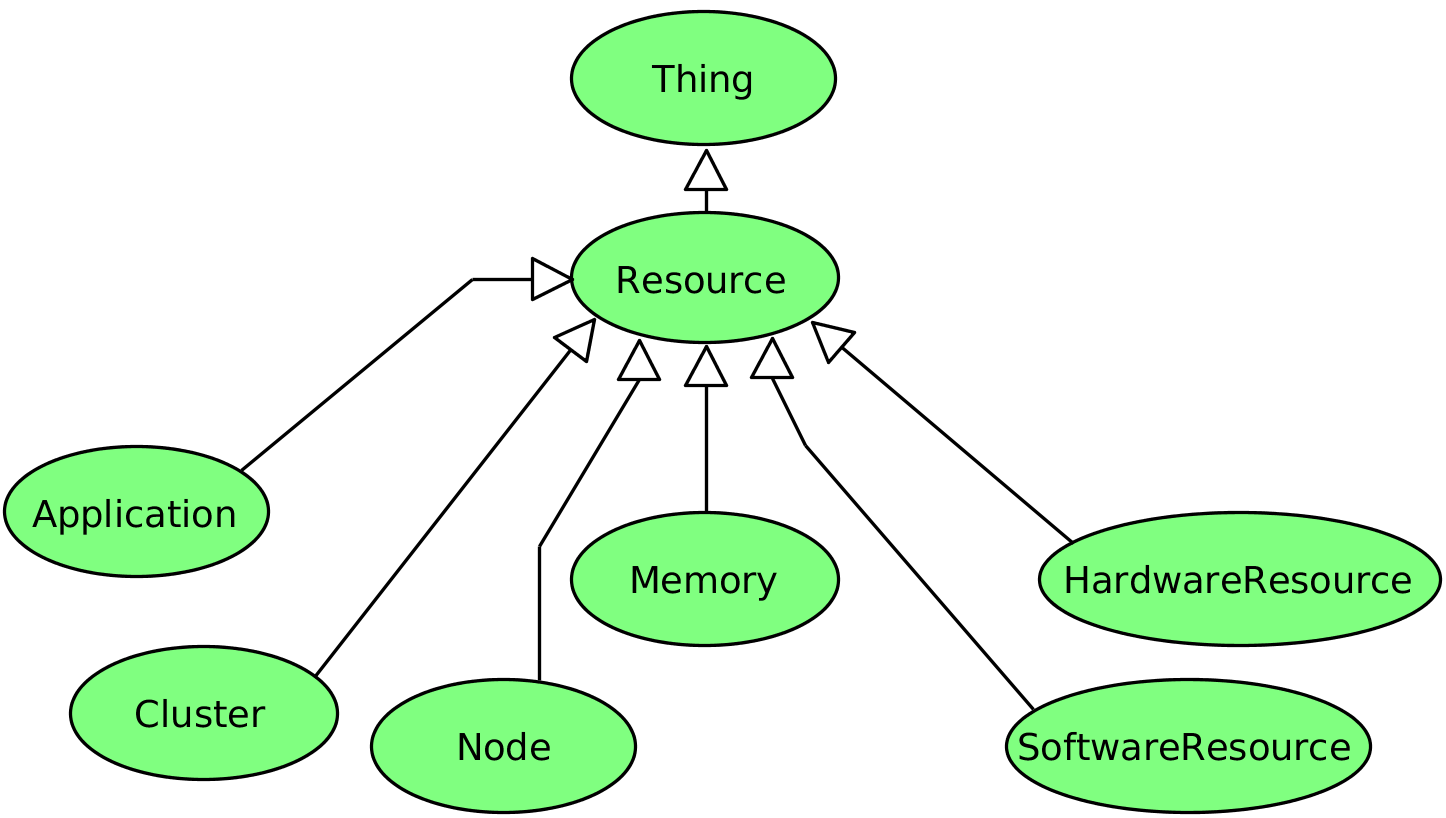
\includegraphics[width=0.6\textwidth]{onto_resources_admin}
\caption{Diagram of is-a (rdfs:subClassOf) relationship between most general resource concepts}
\label{fig:onto_resources_admin}
\end{figure}

Figure~\ref{fig:onto_resources_admin} depicts is-a relationship between general SemSimMon concepts. The root class of every entity in OWL compliant ontologies is owl:Thing, as specified in OWL language reference\cite{owlRef:2004}. To cover all possible resources - generic Resource class was introduced. It acts as a root concept for all other resources and the only one that is direct subclass of owl:Thing. Resource has 6 direct subtypes: Application, Cluster, Node, Memory, HardwareResource and SoftwareResource. Application and Cluster types are so called \lq\lq{}management\rq\rq{} class resources - they doesn't represent actual components, which can be used to perform computations. Instead, they can be used to aggregate one or more elements, which allows user to building more manageable measurement structures. Application is most important item, in context of has-a relationship, which illustrates Figure~\ref{fig:onto_resources_has_a_admin}. It represent program created by user, which He or She wants to analyze using proposed tool. Each application, in theoretical model may be running on multiple clusters, and multiple nodes.

Cluster refers to group of computing nodes which are connected using high efficiency network, thus in some way may be treated as single entity. It is equivalent of site in OMIS nomenclature\cite{tl9702e}. Node can be interpreted as a bridge between high-level resources and software, hardware resources. Generally speaking, it is smallest independent computing unit, e.g. single PC or unit in a rack. It can be treated as administrative type of resource, as it's not a component that is used directly to aid computations, it rather aggregates such a components (all its hardware with operating system). But, on the other hand, node is an actual device that is used in processing. 

There exists also special class of resources - Memory. It's extracted to subclass Resource type directly, because there exists at least two types of memory: software based (virtual memory) and hardware (physical memory) that share common semantics.

\begin{figure}[ht]
\centering
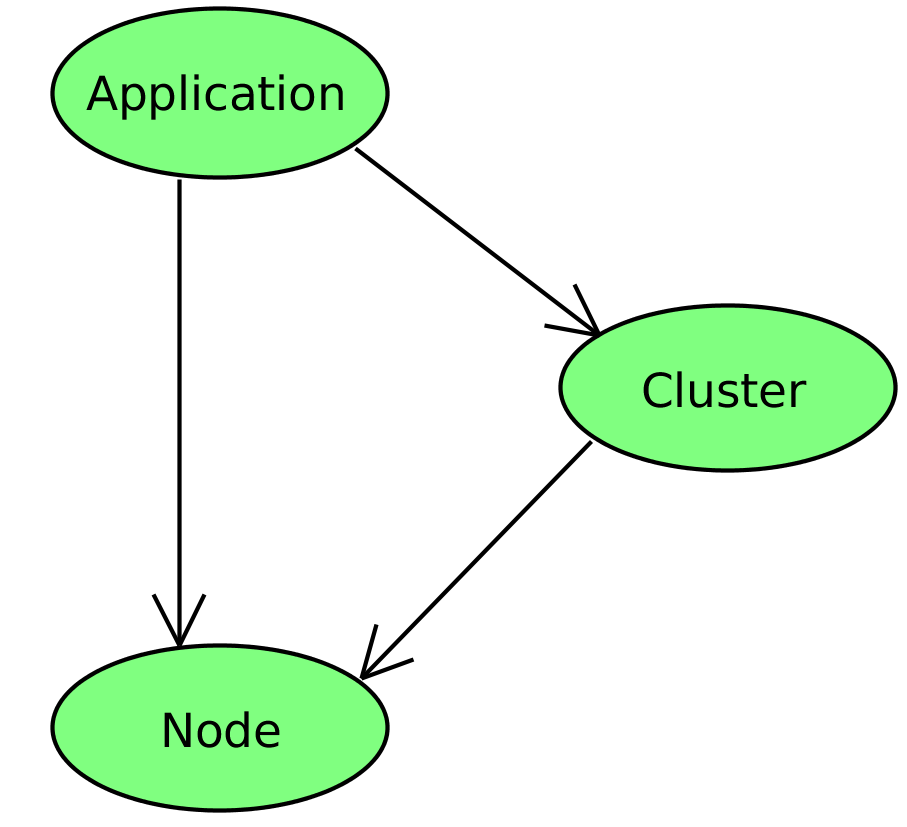
\includegraphics[width=0.3\textwidth]{onto_resources_has_a_admin}
\caption{Diagram of has-a relationship between most general resource concepts}
\label{fig:onto_resources_has_a_admin}
\end{figure}

\pagebreak

\begin{figure}[ht]
\centering
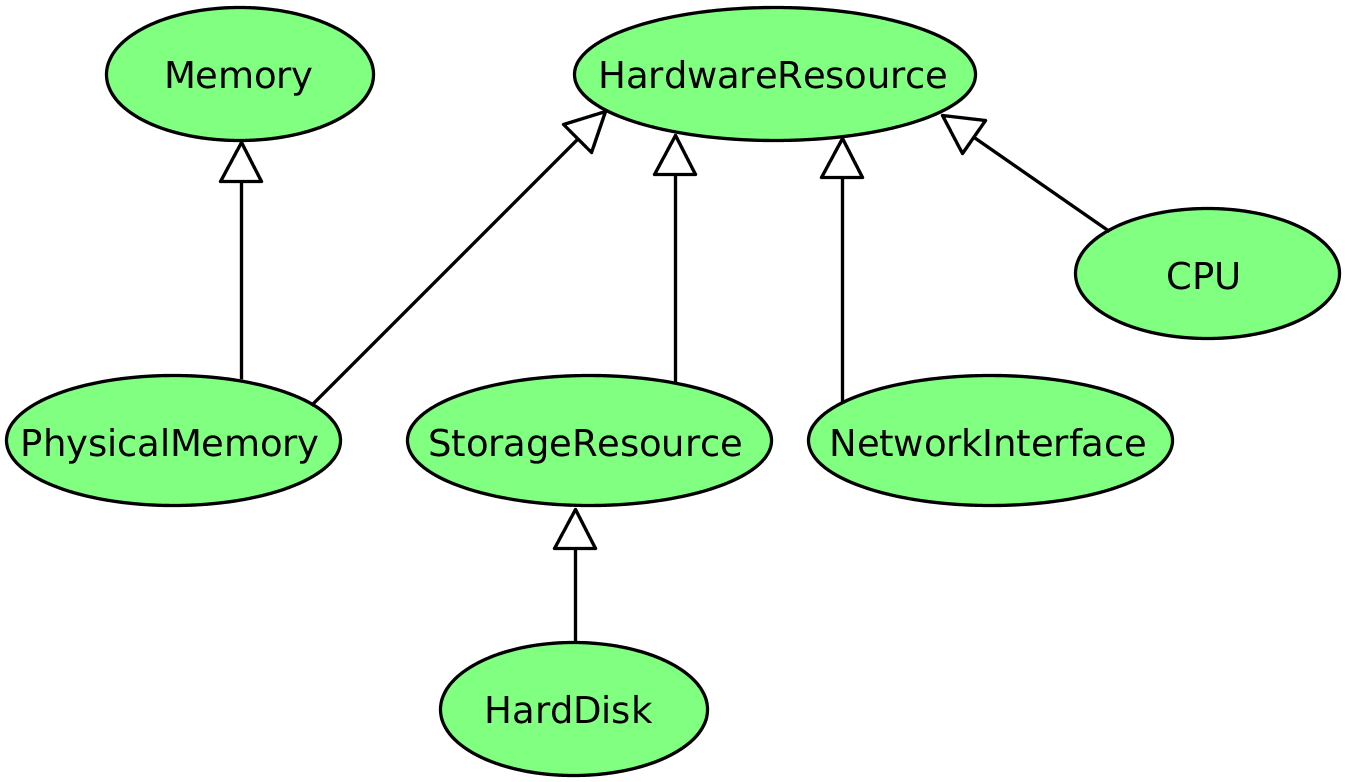
\includegraphics[width=0.6\textwidth]{onto_resources_hardware}
\caption{Diagram of is-a relationship between hardware resources}
\label{fig:onto_resources_hardware}
\end{figure}

Classes related to hardware resources, can be seen in Figures~\ref{fig:onto_resources_hardware} and~\ref{fig:onto_resources_has_a_hardware}. All of them were designed in a way that will allow covering most of computer parts available nowadays on market. Both diagrams are quite straightforward. HardwareResource has 4 direct sub-types: PhysicalMemory, StorageResource, NetworkInterface and CPU. PhysicalMemory, is also subtype of Memory class, to share common semantics, as was stated before. Also, StorageResource has one deriving class - HardDisk. Hardware resources has-a relationship diagram is even more elementary - Node may have all hardware resources, and there are no other relations between those resources. 

\begin{figure}[ht]
\centering
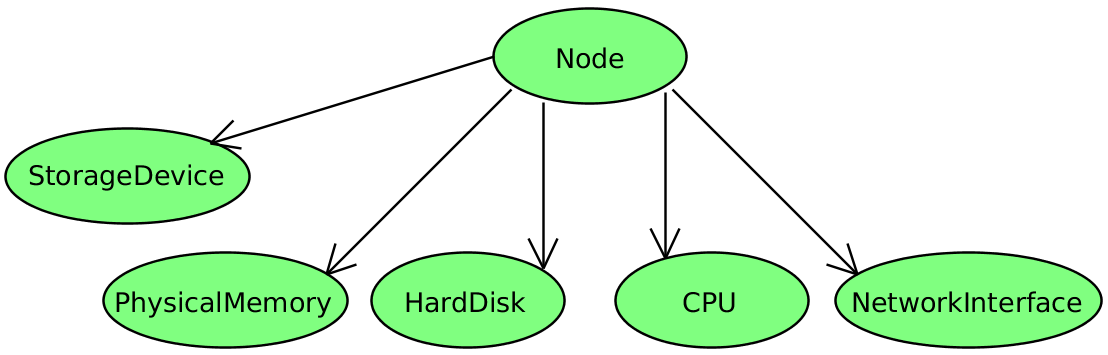
\includegraphics[width=0.7\textwidth]{onto_resources_has_a_hardware}
\caption{Diagram of has-a relationship between hardware resources}
\label{fig:onto_resources_has_a_hardware}
\end{figure}

\begin{figure}[ht]
\centering
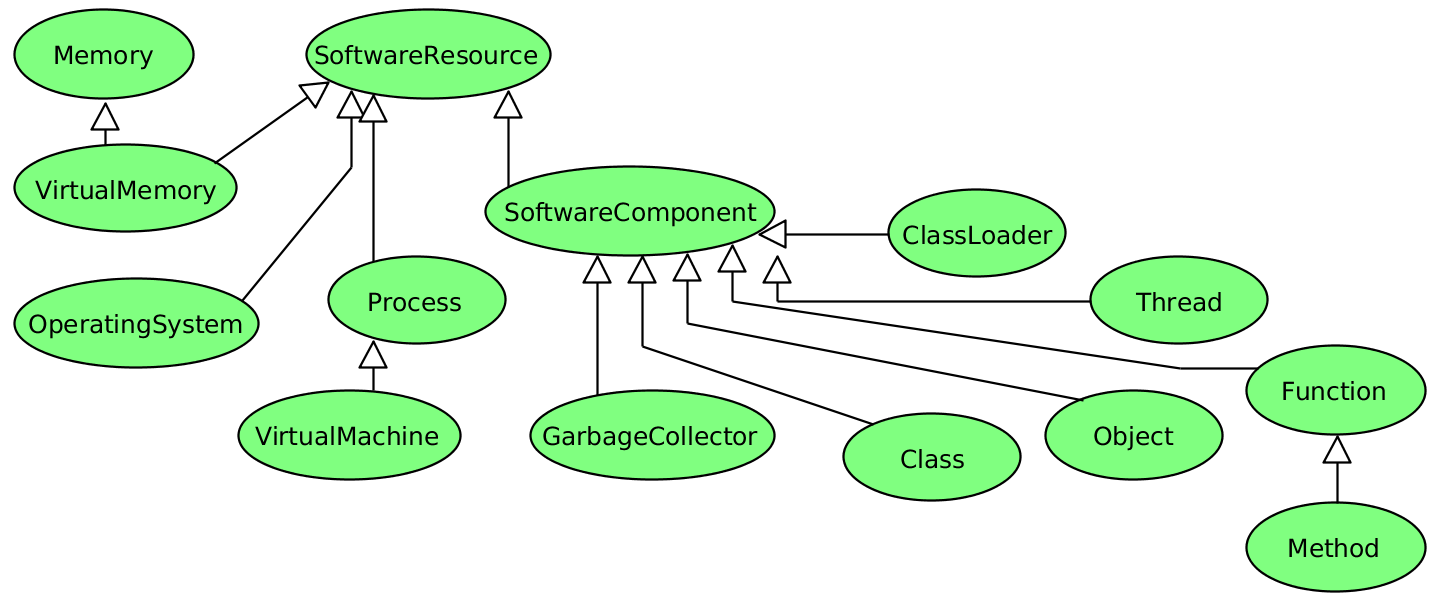
\includegraphics[width=0.9\textwidth]{onto_resources_software}
\caption{Diagram of is-a relationship between software resources}
\label{fig:onto_resources_software}
\end{figure}

System is aware of more software resource types then hardware ones. This implies more sophisticated relationships between those concepts, which are depicted in Figures~\ref{fig:onto_resources_software} and~\ref{fig:onto_resources_has_a_software}. Class SoftwareResource has 4 direct subtypes: VirtualMemory (which also derives from generic Memory concept), OperatingSystem, Process and SoftwareComponent concept. First three types are quite straightforward and represent what one expects them to do. Special subtype of Process, namely VirtualMachine needs more concern. It was extracted from more general type, because of its specific nature which differs it from all general purpose processes. Each virtual machine acts as runtime environment for running application, thus it has specific features common for all virtual machines, but unlikely seen in casual process. SoftwareComponent resource type is logical wrapper for all low level software components that can be used to create program. There are generic components, like Thread, Function. There are also types specific to Object Oriented Programming: Class, Object, and Method (which subtypes Function). The third group of SoftwareComponents subtypes is specific to virtual machines. It contains only two items: GarbageCollector and ClassLoader.

Regarding ownership relations in software category there is one root concept - Node. Each node has: OperatingSystem, and multiple Processes. Some processes may be VirtualMachines, thus this resource is last type that Node may own. Each process may have following software components: Thread, Object, Class and Function. VirtualMachine may have all components that generic process has, and also, two specific: ClassLoader and GarbageCollector. Additionally, Class type owns one type of resource: Method. OperatingSystem resource may have only one software resource type, namely VirtualMemory.

\begin{figure}[ht]
\centering
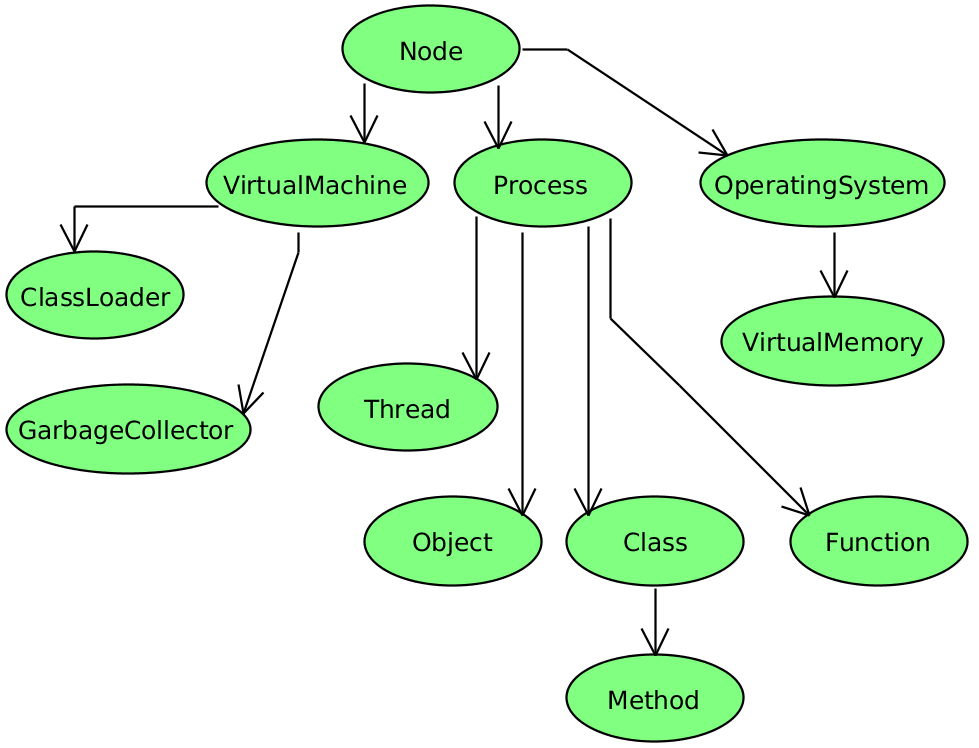
\includegraphics[width=0.7\textwidth]{onto_resources_has_a_software}
\caption{Diagram of has-a relationship between software resources}
\label{fig:onto_resources_has_a_software}
\end{figure}

\pagebreak

\subsection{Capabilities ontology}
\label{subsec:arch_knowledge_capabilitie}

For concepts related to capabilities of resources, only is-a relationship was defined, which can be seen in Figure~\ref{fig:onto_capabilities}. There is one root concept, namely ResourceCapability, which subclasses rdf:Thing. It has 4 direct subtypes: HardwareCapability, MemoryCapability, NodeCapability and SoftwareCapability. For hardware capability, there are only 2 deriving classes StorageCapability and CpuCapability. Since concept of VirtualMemory and PhysicalMemory are semantically close, there is no need to subclass generic MemoryCapability, thus this type doesn't have any subtypes. NodeCapability is another direct subtype of most generic ResourceCapability, which doesn't require any additional child types. 

Complex structure of software resources influences relationships between capabilities related to those components. SoftwareCapability has 3 subtypes: OperatingSystemCapability, ProcessCapability and SoftwareComponentCapability. Additionally, VirtualMachineCapability was extracted from ProcessCapability, because of same reasons that motivate extraction of VirtualMachine resource type from Process - different semantics. The only one type that extends SoftwareComponentCapability is ThreadCapability.

\begin{figure}[ht]
\centering
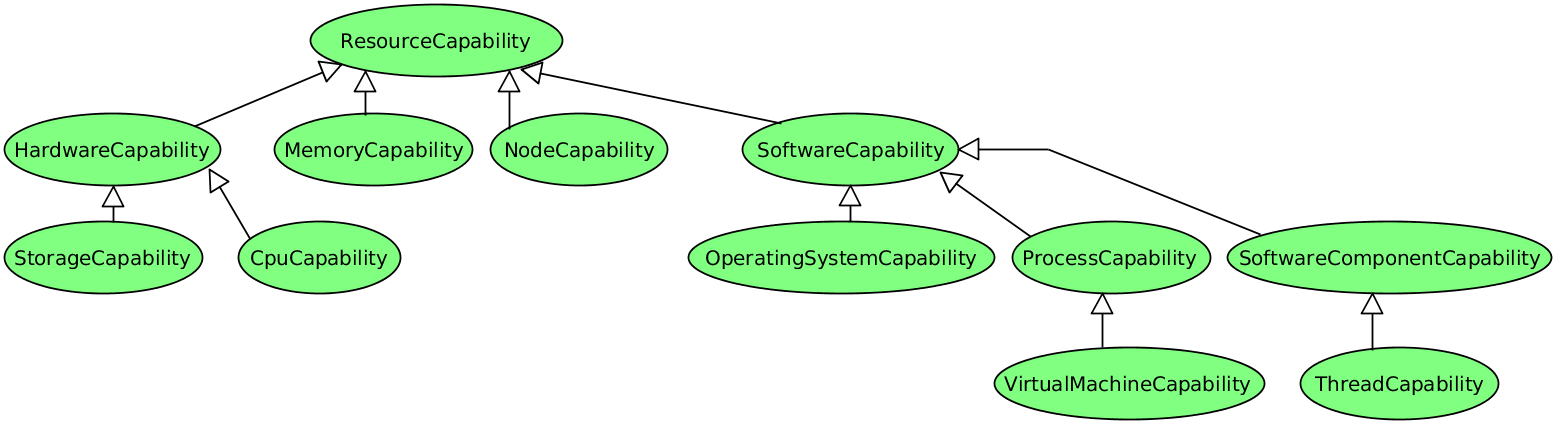
\includegraphics[width=1.0\textwidth]{onto_capabilities}
\caption{Diagram of is-a relationship between capabilities}
\label{fig:onto_capabilities}
\end{figure}

